\begin{ledgroupsized}[r]{120mm}
\footnotesize 
\pstart 
\noindent\textbf{\"{U}berlieferung:}
\pend
\end{ledgroupsized}
\begin{ledgroupsized}[r]{114mm}
\footnotesize 
\pstart \parindent -6mm
\makebox[6mm][l]{\textit{l}}%
Reinschrift von Schreiberhand einer unbekannten Vorlage: LH XXXV 10, 9 Bl. 3-4. 1~Bog. 2\textsuperscript{o}. \nicefrac{1}{2} S. auf Bl.~3~v\textsuperscript{o}. Der Bogen überliefert ferner N.~28\textsubscript{2}, N.~28\textsubscript{5}, N.~28\textsubscript{6} und N.~5.
%LH35,10,09 Bl. 3r = Demonstratio geometrica de magnetis sphaera
\\
Cc 2, Nr. 1190 D
\pend
\end{ledgroupsized}

%%\normalsize
%\vspace*{5mm}
%\begin{ledgroup}
%\footnotesize 
%\pstart
%\noindent\footnotesize{\textbf{Datierungsgr\"{u}nde}: bislang nur relative Chronologie etabliert, absolute Datierung noch ausstehend.}
%\pend
%\end{ledgroup}
\vspace*{8mm}

\pstart 
\normalsize
\noindent
[3~v\textsuperscript{o}]
\pend
\pstart
\centering
\noindent
Regle pour calculer la force d'une machine,\protect\index{Sachverzeichnis}{machine}\protect\index{Sachverzeichnis}{force}\\%
dont voicy la figure
\pend
\vspace{1.0em}
\pstart
\noindent Soit la roue\protect\index{Sachverzeichnis}{roue} \textit{ABCD} mobile \`{a} l'entour du centre \textit{L}. Supposons qu'elle change sa situation perpendiculaire en inclin\'{e}e, dans un angle donn\'{e} \`{a} l'Horison \textit{DB}. S\c{c}avoir dans l'angle \textit{ELB} en sorte que \textit{A} soit trans\-port\'{e} en \textit{E}, et \textit{B} en \textit{F}, et \textit{C} en \textit{G}, et \textit{D} en \textit{H}.\\ \indent Dans les Rayons \textit{LH}, et \textit{LG} soyent prises les droites egales entre elles, \textit{LI} et \textit{LK} moindres que les Rayons, mais dans une certaine raison connue, ou donn\'{e}e.
\pend
\vspace{1.5em}
\pstart
\noindent
\centering
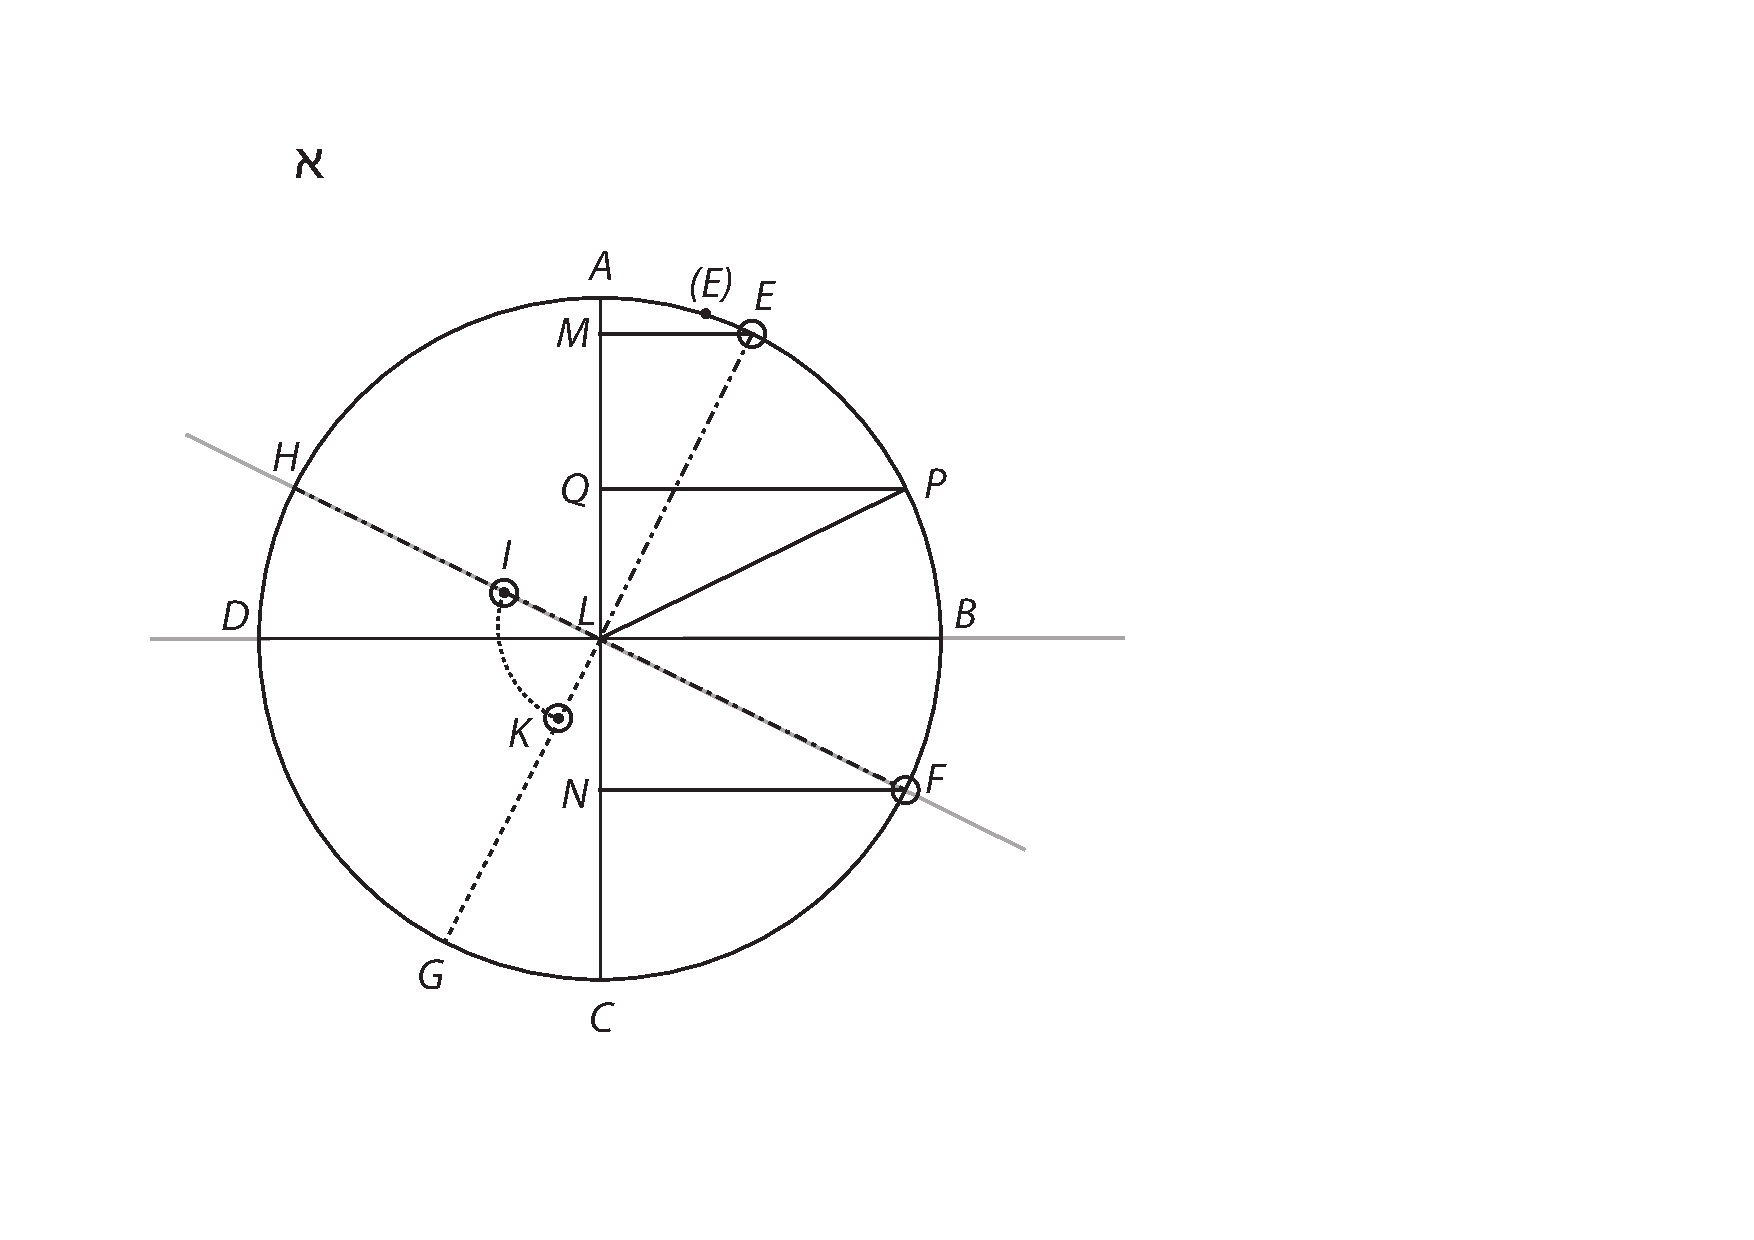
\includegraphics[trim = 0mm -3mm -2mm 0mm, clip, width=0.62\textwidth]{images/lh0351009_003v-d1.pdf}\\
\noindent \setline{11}\centering [\textit{Fig. 1}]
\pend
\newpage
\pstart Supposons \`{a} present 4 poids egaux entre eux, appuyez ou suspendus dans les points \textit{E. F. K.} \edtext{[\textit{I.}]}{\lemma{}\Bfootnote{\textit{L.} \textit{l \"{a}ndert Hrsg.}}}\\ \indent Enfin soit donn\'{e} la force absolue auec laquelle d'un tel poids\protect\index{Sachverzeichnis}{poids}.
\pend 
%\newpage
\pstart J'appelle la force absolue auec laquelle il agit librement; s\c{c}avoir auec laquelle un poids agit sur un plan parallele \`{a} l'horison, qui le soutient.
\pend 
\pstart Cela pos\'{e}, le calcul se fera ainsy.
\pend 
%\newpage
\pstart Du point \textit{E} menez la perpendiculaire \textit{EM}, sur le diametre \textit{AC}, perpendiculaire \`{a} l'horison \textit{DB}, laquelle sera le sinus droit de l'Angle \textit{ALE}.\pend \pstart Appellons 
\begin{tabular}[t]{lcr}
le sinus droit &\textit{EM},&\textit{y}\\
le {Rayon\reversemarginpar\marginnote{\scriptsize\hspace{-13mm}10}} &\textit{AL},&\textit{a}\\
le Rayon&\textit{LI}, ou \textit{LK},&\textit{b}\\
\multicolumn{2}{l}{la force absolue du poids,}&\textit{g}\\
\end{tabular} 
\pend 
\vspace{0.3em}
\pstart \noindent et \setline{13}\textso{la force de la machine}\protect\index{Sachverzeichnis}{machine} sera \rule[-4mm]{0mm}{10mm}${\displaystyle \frac{yag + ag\sqrt{a^2 - y^2} - gby - gb\sqrt{a^2 - y^2}}{ba}}$, ou $y + \sqrt{a^2 - y^2}, \smallfrown \displaystyle\frac{a}{b} - 1, \smallfrown \displaystyle\frac{g}{a}$\rule[-4mm]{0mm}{10mm}. 
\pend 
\pstart C'est \`{a} dire, prennez la somme de \textit{ME} et \textit{ML}; et la multipliez par \rule[-4mm]{0mm}{10mm}$\displaystyle\frac{a}{b} - 1$; et le produit, par \rule[-4mm]{0mm}{10mm}$\displaystyle\frac{g}{a}$. Ce qui en proviendra, sera la force de la machine,\protect\index{Sachverzeichnis}{force} en quelque situation qu'elle puisse estre. 
\pend